\section{Schedulering}

\begin{figure}[h!]
	\centering
	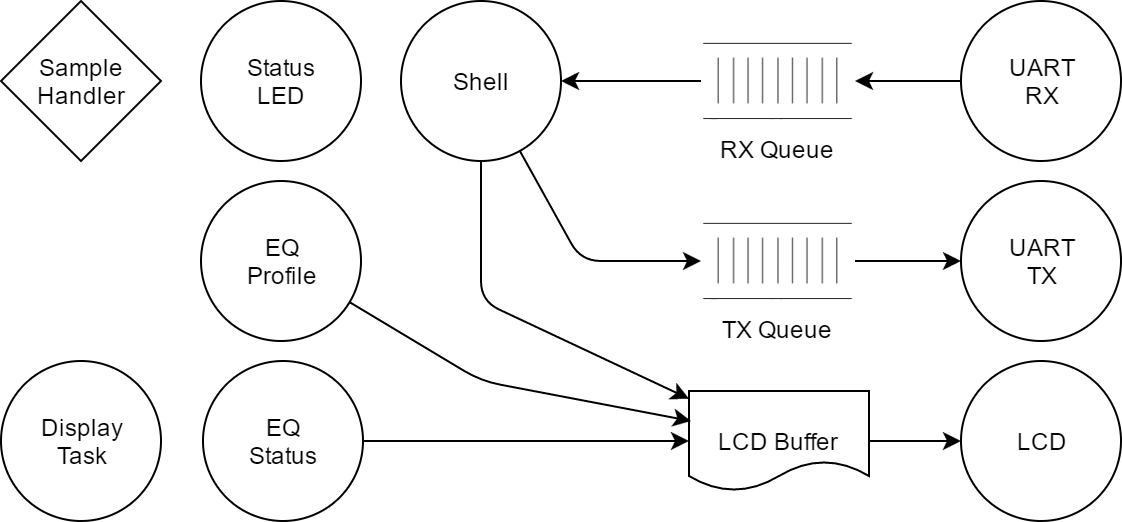
\includegraphics[width=.8\textwidth]{billeder/eq-one.png}
	\caption{Task model af equalizerens operativ system.}
	\label{fig:eq-taskmodel}
\end{figure}

Task diagram af interrupt vs. schedulering.

Forklar (diagram) algoritmen for scheduleringen. Prioritet af tasks, etc.

State diagram af schedulering.

Argumentere og for at systicks ikke misses pga. int. prioritering og at sceduleringen kan tage højde for dette.

Overbevis læseren om at scheduleringen er effektiv til formålet .

Noter:
Problemer med schedulring når der ikke er tid til de enkelt tasks inden for et tick, når eq bliver aktiveret bliver der endnu mindre tid og så sker det at der misses ticks.
Tag tider når OS starter op uden EQ tændt, og sammenlign med tider når EQ kører, så er tiden hver task er om at kører inkl. den tid som audio int. bruger -> nu skrider hele scheduleringen og tick misses. Især når eq-profil-amp funktionen bruges, som tager meget lang tid.

Optimalt at flytte eq-profil dannelsen ind i boot sec. så den ikke bruger tid i realtime.

Tiderne på LOW, MEDIUM og HIGH prioritet har indflydelse på systemet, absolut ikke den bedste løsning, en preemptive schedulering ville helt klart afhjælpe nogle af de problemer.




 

